\documentclass[10pt, twocolumn]{article}
\usepackage{url}
\usepackage{color,graphicx}
\usepackage{amssymb,amsmath,amsthm,subfigure}
\usepackage[numbers]{natbib}
\usepackage{algorithm2e}
\usepackage{almostfull}

%%% Environment for notation and a symbol command to go along with it.
%%% The argument should be the widest symbol which is expected if 
%%% \sym will be used to make the list.
%%%
\newenvironment{notation}[1]{%
\begin{list}{}{\small
\settowidth{\labelwidth}{{#1}\quad}%
\setlength{\itemsep}{1.5pt plus 0.5pt minus 0.2pt}%
\setlength{\parsep}{0ex}%
\setlength{\rightmargin}{0em}%
\setlength{\leftmargin}{\labelwidth}%
\addtolength{\leftmargin}{\labelsep}%
\addtolength{\leftmargin}{1em}}}{\end{list}}

\newcommand{\sym}[1]{\item[${#1}$\hfill{}]}

\newcommand{\bx}{\mathbf{x}}
\newcommand{\bu}{\mathbf{u}}
\newcommand{\tx}{\tilde{x}}
\newcommand{\norm}[1]{\vert #1 \vert}
\newcommand{\set}[1]{\left\lbrace #1 \right\rbrace}
\newcommand{\SetAlgoLined}{}

\newcommand{\I}{\mathcal{I}}
\newcommand{\BO}{\textrm{BO}}
\newcommand{\IP}{\textrm{Ip}}
\newcommand{\UP}{\textrm{Up}}
\newcommand{\DN}{\textrm{Dn}}
\newcommand{\Inv}{\textrm{Iv}}
\newcommand{\Dem}{\textrm{Dm}}
\newcommand{\ulambda}{\underline{\lambda}}
\newcommand{\olambda}{\overline{\lambda}}
\newcommand{\eig}{\text{eig}}
\newcommand{\diag}{\text{diag}}

\newtheorem{assumption}{Assumption}
\newtheorem{definition}{Definition}
\newtheorem{proposition}{Proposition}
\newtheorem{theorem}{Theorem}
\theoremstyle{definition}
\newtheorem{algo}{Algorithm}

\title{Cooperative  model predictive control: Current status and  limitations }
\author{Kaushik Subramanian \thanks{Department of Chemical and Biological
     Engineering, University of Wisconsin-Madison, U.S.A.}  \and James
  B. Rawlings\footnotemark[1] \thanks{Corresponding author: rawlings@engr.wisc.edu}}  


\begin{document}
\maketitle
\section{Introduction}

\section{Preliminaries}
\label{sec:prelim}
In this section, we describe the system under study and the different
constraint sets and objective functions employed for developing the
centralized and cooperative model predictive controllers. We also introduce a
simple two--tank example used throughout the paper to illustrate the
properties of the proposed cooperative controller.

In this paper, we develop cooperative controllers for an overall system comprising of two subsystems. However, the algorithms presented can be easily extended to centralized problems consisting of multiple subsystems.
\paragraph {\textbf{System.}} We consider linear systems comprising of two subsystems  of the form 
\[ \begin{bmatrix}x_1\\x_2\end{bmatrix}^+ = \begin{bmatrix}A_1& \\ & A_2\end{bmatrix}\begin{bmatrix}x_1\\x_2\end{bmatrix}+ \begin{bmatrix}B_{11}\\B_{21}\end{bmatrix}u_1 + \begin{bmatrix}B_{21}\\B_{22}\end{bmatrix}u_2
\]
in which $x = (x_1,x_2)$ and $u = (u_1,u_2)$ are the overall (centralized) system states and inputs. Subsystem-$i$ manipulates input $u_i$ and consists of states $x_i$. Note that the states are affected by inputs from both subsystem. We make the following assumption on the centralized system.
\begin{assumption}
\label{ass:stab}
The centralized system $(A,B) = \begin{bmatrix}A_1& \\ & A_2\end{bmatrix}, \begin{bmatrix}B_{11}& B_{21}\\B_{12} & B_{22}\end{bmatrix}$ is stabilizable. 
\end{assumption}
\paragraph {\textbf{Constraints.}} The input and state constraints satisfy the following assumption.
\begin{assumption}
\label{ass:const}
There are no state constraints and the input constraints are uncoupled. Input $u_i$ is constrained to lie in a convex, compact set containing the origin in its interior, $\mathbf{U}_i$. For the centralized system, we denote the input constraint set $\mathbf{U} = \mathbf{U}_1 \times \mathbf{U}_2$.
\end{assumption}

\paragraph{\textbf{Stage costs.}} To each subsystem, we assign the stage cost
\[ \ell_i(x_i,u_i) = x_i'Q_ix_i + u_i'R_iu_i \qquad  i = \set{1,2} 
\]
in which $Q_i,R_i$ are positive definite matrices for each subsystem. The overall (centralized) cost function is $\ell(x,u) = \ell_1(x_1,u_1)+\ell_2(x_2,u_2)$. We define $Q = \begin{bmatrix} Q_1 & \\ & Q_2 \end{bmatrix}$ and $R = \begin{bmatrix} R_1 & \\ & R_2 \end{bmatrix}$ so that the stage cost for the centralized system can be written as $\ell(x,u) = x'Qx+u'Ru$. 

\paragraph {\textbf{Terminal penalty and terminal set.}} Since the centralized system is stabilizable (from Assumption \ref{ass:stab}) and the stage costs are positive definite, there exists a controller gain $K = \begin{bmatrix} K_1\\K_2\end{bmatrix}$ such that the closed-loop system $x^+ = (A+BK)x$ is stable. In other words, all the eigen-values of $(A+BK)$ lie inside the unit circle. Associated with the gain $K$ is the positive definite matrix $P$, that is the solution to the Lyapunov equation
\[ A_K'PA_K + Q_K = P; \qquad A_K = (A+BK), Q_K = Q+K'RK\]
We use $P$ as the terminal penalty $V_f(x) = x'Px$. 

For the pair $(P,K)$, we can define the control invariant  region in state-space in which the controller $u=Kx$ does not activate any input constraints. 
\[ \mathbb{F}:= \set{x \mid x^+ = (A+BK)x \in \mathbb{F}, u = Kx \in \mathbf{U}} \]

We denote the set $\mathbb{F}$, which is a closed set containing the origin in its interior  as the terminal region. For linear systems, the set $\mathbb{F}$ is polytopic.

We also denote the following set $\mathbb{E}$ which is a level set of the terminal penalty as the terminal region, parametrized by the parameter $a>0$.
\[ \mathbb{E}:= \set{V_f(x) \leq a}
\]

For any $a>0$ such that $\mathbb{E} \subset \mathbb{F}$, the set
$\mathbb{E}$ can also be used as the terminal set. The set
$\mathbb{E}$ is an ellipsoidal region in $\mathbb{R}^{n}$, in which
$n$ is the dimension of the state.

We denote $\mathbb{T} \subset \mathbb{R}^n$ to be the following set
\[ \mathbb{T} := \set{0} \]

\textbf{Remark.} Note that the terminal region and terminal penalty is defined only in terms of the centralized state and input $(x,u)$. We could define such regions and penalties for individual subsystems if the pair $(A_i,B_i)$ were stabilizable. For the cooperative MPC algorithms in this paper, however, we impose no assumptions on the stabilizability of the subsystems.

\paragraph{\textbf{Cost functions.}} We define the following objective functions. We define $N$ as the prediction/control horizon and the vector $\bu$ as $\bu = (u(0),u(1),\ldots,u(N-1))$. 
The cost function $V_N(x,\bu)$ is the sum of the $N$ stage costs and the terminal cost.
\[V_N(x,\bu) = \sum_{k-0}^{N-1} \ell(x(k),u(k)) + V_f(x(N)) \]


\paragraph{\textbf{Optimization problems.}} We define the following
optimization problem based on different terminal constraint regions.
\begin{enumerate}
\item {\em{Terminal control:}} In the terminal control problem, we
  constrain the state at the end of the prediction horizon to be at
  the origin. 

\begin{align*} \mathbb{P}_N^{\mathbb{T}}(x) &: \min_{\bu}{V_N(x,\bu)}\\ &
  \text{~s.t~} x^+ = Ax+Bu,\\& \bu \in \mathbf{U}^N,\\& x(N) \in
  \mathbb{T} \end{align*}

\item {\em{ Terminal region control:}} In terminal region control, we constrain the final state $x(N)$ to lie in a terminal region. We define two terminal region control optimization problems, one each corresponding to the polytopic terminal region $\mathbb{F}$ and the ellipsoidal terminal region $\mathbb{X}_f$.
\begin{align*}\mathbb{P}_N^{\mathbb{F}}(x) &: \min_{\bu}{V_N(x,\bu)} \\& \text{~s.t~} x^+ = Ax+Bu,\\& \bu \in \mathbf{U}^N,\\& x(N) \in \mathbb{F} \end{align*}
\begin{align*} \mathbb{P}_N^{\mathbb{E}}(x) &: \min_{\bu}{V_N(x,\bu)}\\& \text{~s.t~} x^+ = Ax+Bu,\\& \bu \in \mathbf{U}^N,\\& x(N) \in \mathbb{E} \end{align*}

\end{enumerate}
%\paragraph{\textbf{Region of attraction.}} The region of attraction of a MPC controller is the region of the state-space in which the optimization problem solved on-line by the controller is feasible. For example, for the terminal region con%troller, the region of attraction $\mathcal{X}_N^\mathbb{F}$ is given by:
%\[\mathcal{X}_N^\mathbb{F}:= \set{x \mid \exists \bu \in \mathbf{U}^N \text{~s.t~} \phi(N;x,\bu) \in \mathbb{F}}
%\]
%in which $\phi(N;x,\bu)$ is $x(N)$ starting from $x$ under control $\bu$. For the different optimization problems mentioned earlier, the region of attraction satisfy the following relationship
%\[ \mathcal{X}_N^\mathbb{F} \supseteq \mathcal{X}_N^{\mathbb{X}_f(a)} \supseteq \mathcal{X}_T
%\]

\paragraph{\textbf{Example.}} The example that we use to study the
different properties of the cooperative MPC controller that we propose
is the two-tank system shown in Figure \ref{fig:2tank}. The system
consists of two tanks, each of which is a separate subsystem for
implementing cooperative MPC. Tank-1 has three valves at its disposal
to manipulate. The valve $u_{13}$ that directly drains water from the
first tank is expensive to manipulate as compared to valve $u_{12}$
that drains water from the first tank into the second tank. Similarly,
the recycle stream is cheaper to manipulate than the direct drain in
the second tank. We assume that at steady state, all the flows are
non-zero, and the levels in the tank are such that, the state
constraints are not active. %Although, all the inputs are constrained
                            %physically to operate between
                            %$[0,\bar{u}]$, with $0$ corresponding to
                            %valves closed and $\bar{u}$ corresponding
                            %to valve open; in deviation variables,
                            %the input constraints include origin,
                            %because of the assumption that all the
                            %flows are non-negative at steady state. 
We also introduce a perfectly modeled disturbance that adds water in the first tank at a rate proportional to the flow out of the second tank $u_{21}$. 
\begin{figure}
\centering
{\resizebox{0.9\columnwidth}{!}{\input{2tanks}}}
\caption{The two-tank system.}
\label{fig:2tank}
\end{figure}
\section{Suboptimal MPC}
We denote the optimiazation problem as $\mathbb{P}(x)$ to refer to any
one of the three optimization problems described in the previous
section.
\[ \mathcal{U}(x) := \set{ \bu \in \mathcal{U}^N \mid (x,\bu) \text{~is feasible for~} \mathbb{P}(x)}
\] 
If we denote $\kappa(x) = \bu^0(0;x)$ as the first element of the optimal solution of the problem $\mathbb{P}(x)$ then we can show that the corresponding optimal value function $V^0(x,\bu^0(x))$ is a  Lyapunov function for the closed-loop dynamics $x^+ = Ax +B\kappa(x)$, following the theory outlined in \citep[Chapter 2]{rawlings:mayne:2009}. Lyapunov theory then helps us to establish (a) asymptotic (exponential for linear systems) convergence to the origin and, (b) stability of the closed loop $x^+= Ax+B\kappa(x)$. 

However, as the name suggests, in suboptimal MPC, we do not inject $\kappa(x)$ as the input to the plant. Instead, we wish to inject {\emph{some}} feasible input to the plant. In order to ensure that despite injecting suboptimal inputs to the plant, we maintain the close-loop properties of optimal MPC, we define the warm start and the successor input set that ensures that the closed-loop suboptimal MPC has the desired properties. We define $\kappa_s(x)$ as the first input in the suboptimal input sequence.
\begin{definition}[Warm Start]
\label{def:warmstart}
Let $(x,\bu)$ be a state-input vector pair such that $\bu$ is feasible for $\mathbb{P}(x)$. Then the warm start for the successor initial state
$x^+ = Ax+B\kappa_s(x)$ is defined as:
\begin{equation*}
%\label{eq:warmstart}
\tilde{\bu} = \left (\bu(1;x),\bu(2;x),\ldots,\bu(N;x),u_+\right)
\end{equation*}
in which  $u_+ = K\phi(N;x,\bu)$.
\end{definition}
\begin{definition}[Successor input set]
\label{def:G}
Consider $(x,\bu)$ such that $\bu$ is feasible for $\mathbb{P}(x)$. For the  successor state
$x^+ = Ax+B\kappa_s(x)$, we define the set $G(x,\bu)$
\begin{multline*}
G(x,\bu) = \lbrace \bu^+ \mid \bu^+ \in
\mathcal{U}(x^+), V(x^+,\bu^+)\leq V(x,\tilde{\bu}), \\
V(x^+,\bu^+) \leq V_f(x^+) \text{~if~} x\in r\mathbb{B} \rbrace
\end{multline*}
in which $\tilde{\bu}$ is the warm start given by Definition 
\ref{def:warmstart} and $r\mathbb{B}$ is a ball of radius $r>0$. We choose $r$ sufficiently small such that $r\mathbb{B}$ is a subset of the terminal region. We can show that this constraint is equivalent to  $\bu \leq d \norm{x}, x \in r\mathbb{B},d >0$. For terminal constraint MPC, we implement the second constraint.  
\end{definition}
\begin{theorem}
\label{thm:suboptimal}
Let Assumptions \ref{ass:stab} and \ref{ass:const}
hold. Choose optimization problem $\mathbb{P}(x) \in \set{
  \mathbb{P}_N^{\mathbb{T}}(x), \mathbb{P}_N^{\mathbb{F}}(x),
  \mathbb{P}_N^{\mathbb{E}}(x)}$ and the appropriate terminal
regions. For any $x$ for which  $\mathcal{U}(x)$  is not empty, choose $\bu \in \mathcal{U}(x)$. Then, the origin of the closed-loop system
\begin{align*}
x^+ &= Ax+ B\kappa_s(x) \\
\bu^+ &\in G(x,\bu)
\end{align*}
is asymptotically stable on (arbitrarily large) compact  subsets of
the feasible region $\mathcal{X}_N :=\set{x\mid \exists u \in
  \mathbf{U}^N, \text{~s.t~} \mathcal{U}_N(x) \neq \varnothing}$. 
\end{theorem}

The proof of Theorem \ref{thm:suboptimal} is presented in \citep{pannocchia:rawlings:wright:2011}.

Observe that for the nominal system, the warm start is a member of the set $G(x,\bu)$. Therefore, if we have a feasible $(x,\bu)$ pair, we can construct an asymptotically stable closed loop without any optimizations. However, if we wish to improve performance by optimizations, we need the optimization algorithm to have the following properties:
\begin{definition}
\label{thm:propO}
The optimization algorithm $\mathbb{O}$ applied to $\mathbb{P}(x)$ has the following properties:
\begin{enumerate}
\item It is an iterative algorithm starting from a feasible point $(x,\tilde{\bu})$.
\item Every iteration $\bu$ decreases the objective function. 
\item Every iteration is feasible.
\end{enumerate}
\end{definition}
Properties (2) and (3) ensure that {\em{any intermediate iterate}} generated by algorithm $\mathbb{O}$ belongs to the set $G(x,\bu)$. Hence, we need not  wait for the optimizations to converge and can inject the suboptimal input from any iterate to the plant without compromising the closed-loop properties.

\textbf{Remark.} We have to include the constraint $V(x,u) \leq V_f(x), \text{~if~} x \in r\mathbb{B}$ in the optimization problem $\mathbb{P}(x)$ to ensure stability of suboptimal MPC. However, since $r$ can be chosen arbitrarily small, this constraint becomes active only asymptotically. Hence, for practical purposes, we do not include this constraint in the optimization problem.


\textbf{Remark.} The properties of the optimizer given by Definition \ref{thm:propO} means that not all optimization algorithms is suitable for suboptimal MPC. For example, optimizers minimizing an augmented Lagrangian function achieve feasibility only at convergence and hence the intermediate iterates are infeasible. Such optimizers are not suitable for suboptimal MPC. 

In section \ref{sec:relax}, we use Theorem \ref{thm:suboptimal} to prove stability of the cooperative MPC algorithm.

\section{Distributed MPC}
In a networked system, there are many interconnected subsystems with each subsystem running its own MPC. These local MPC's optimize a {\emph{local}} objective function that penalizes the local states and the inputs. However, since the subsystems are interconnected by mass and energy balances, the local objective function values depends on decisions made in other subsystems as well. Consider a plant with two subsystems as described in Section \ref{sec:prelim}. Subsystem-$1$ MPC solves the following problem
\begin{align*} \mathbb{P}_1(x;\bu_2)&: \min_{\bu_1} {V_1(x_1,\bu_1)}\\& \text{~s.t~} \bu_1 \in \mathbf{U}_1^N, x_1^+= A_1x_1+B_{11}u_1+B_{21}u_2\end{align*}
We can observe that the value function $V_1(x_1,\bu_1)$ depends on $\bu_2$, decisions made by subsystem-$2$. The objective of distributed MPC is to coordinate the various MPC's.

In noncooperative control, the subsystems share information with each-other. Therefore, subsystem-$1$ shares its predicted input sequence $\bu_1$ with subsystem-$2$ and vice-versa. The subsystem MPC's still solve their local MPC problems. We can view the local MPC with information sharing as feed-forward disturbance rejection, as essentially, subsystem-$1$ MPC is trying to ``reject'' the disturbance injected by subsystem-$2$ inputs. It is easy to see that just sharing information could lead to closed-loop instabilities since the subsystems do not care about the impact of their inputs on other subsystems. In Figure \ref{fig:unstable}, we see that noncooperative MPC destabilizes the two tank system, because, despite having information about the other subsystem inputs, both the tanks manipulate the cheap inputs as their objective functions are not affected by the other subsystem states. However, manipulating the cheap input leads to instability because of the presence of the disturbance. Although subsystem-2 knew about the disturbance, it chose not to manipulate its expensive valve. 

We now consider the situation in which apart from sharing information about their input moves, both the subsystems optimize the overall plant objective. In this case, the subsystem-$1$ MPC problem is:
\begin{align*} \mathbb{P}_1(x;\bu_2)&: \min_{\bu_1} {V_1(x_1,\bu_1)+V_2(x_2,\bu_1)}\\& \text{~s.t~} \bu_1 \in \mathbf{U}_1^N, x^+= Ax+B_{1}u_1+B_{2}u_2\end{align*}
Note that, the size of the subsystem-$1$ optimization problem still remains the same; with the only change in complexity being a new objective function (the equality constraints can be projected out). In this case, it is not immediately apparent that the two subsystem MPC's will not be coordinated and lead to instability. However, merely sharing objective function lead to instability because of poor design of the control problem for unstable systems. For open-loop unstable systems, stability theory of centralized MPC, which has been described in the previous sections gives us design procedures to formulate the optimization problem that needs to be solved at each sampling time to ensure closed-loop properties. If we include these stability constraints in the cooperative MPC problem, we can guarantee closed-loop stability. In such case, the subsystem-$1$ MPC problem is (for terminal constraint MPC):
\begin{align*} \mathbb{P}_1(x;\bu_2)&: \min_{\bu_1}{V_N(x,\bu)} \\&\text{~s.t~}  \bu_1 \in \mathbf{U}_1, x^+=Ax+B_{1}u_1+B_{2}u_2, x(N) = 0 \end{align*}
Similarly, subsystem-$2$ solves
\begin{align*} \mathbb{P}_1(x;\bu_1)&: \min_{\bu_2}{V_N(x,\bu)}\\& \text{~s.t~}  \bu_2 \in \mathbf{U}_2, x^+=Ax+B_{1}u_1+B_{2}u_2, x(N) = 0 \end{align*}

Since both the subsystems are solving a version of the overall optimization problem, cooperative MPC can be viewed as using a decomposition algorithm to solve the optimization problem. To ensure closed-loop stability and asymptotic convergence, we show that the input sequence obtained by solving these two subsystem optimization problems lies in the set $G(x,\bu)$, and hence, use suboptimal MPC theory to establish the closed-loop properties. We use theory developed in Section \ref{sec:relax} to stabilize the cooperative MPC shown in Figure \ref{fig:unstable}.

\begin{figure*}
\centering
\scriptsize
\resizebox{\textwidth}{!}{% GNUPLOT: LaTeX picture with Postscript
\begingroup
  \makeatletter
  \providecommand\color[2][]{%
    \GenericError{(gnuplot) \space\space\space\@spaces}{%
      Package color not loaded in conjunction with
      terminal option `colourtext'%
    }{See the gnuplot documentation for explanation.%
    }{Either use 'blacktext' in gnuplot or load the package
      color.sty in LaTeX.}%
    \renewcommand\color[2][]{}%
  }%
  \providecommand\includegraphics[2][]{%
    \GenericError{(gnuplot) \space\space\space\@spaces}{%
      Package graphicx or graphics not loaded%
    }{See the gnuplot documentation for explanation.%
    }{The gnuplot epslatex terminal needs graphicx.sty or graphics.sty.}%
    \renewcommand\includegraphics[2][]{}%
  }%
  \providecommand\rotatebox[2]{#2}%
  \@ifundefined{ifGPcolor}{%
    \newif\ifGPcolor
    \GPcolortrue
  }{}%
  \@ifundefined{ifGPblacktext}{%
    \newif\ifGPblacktext
    \GPblacktexttrue
  }{}%
  % define a \g@addto@macro without @ in the name:
  \let\gplgaddtomacro\g@addto@macro
  % define empty templates for all commands taking text:
  \gdef\gplbacktext{}%
  \gdef\gplfronttext{}%
  \makeatother
  \ifGPblacktext
    % no textcolor at all
    \def\colorrgb#1{}%
    \def\colorgray#1{}%
  \else
    % gray or color?
    \ifGPcolor
      \def\colorrgb#1{\color[rgb]{#1}}%
      \def\colorgray#1{\color[gray]{#1}}%
      \expandafter\def\csname LTw\endcsname{\color{white}}%
      \expandafter\def\csname LTb\endcsname{\color{black}}%
      \expandafter\def\csname LTa\endcsname{\color{black}}%
      \expandafter\def\csname LT0\endcsname{\color[rgb]{1,0,0}}%
      \expandafter\def\csname LT1\endcsname{\color[rgb]{0,1,0}}%
      \expandafter\def\csname LT2\endcsname{\color[rgb]{0,0,1}}%
      \expandafter\def\csname LT3\endcsname{\color[rgb]{1,0,1}}%
      \expandafter\def\csname LT4\endcsname{\color[rgb]{0,1,1}}%
      \expandafter\def\csname LT5\endcsname{\color[rgb]{1,1,0}}%
      \expandafter\def\csname LT6\endcsname{\color[rgb]{0,0,0}}%
      \expandafter\def\csname LT7\endcsname{\color[rgb]{1,0.3,0}}%
      \expandafter\def\csname LT8\endcsname{\color[rgb]{0.5,0.5,0.5}}%
    \else
      % gray
      \def\colorrgb#1{\color{black}}%
      \def\colorgray#1{\color[gray]{#1}}%
      \expandafter\def\csname LTw\endcsname{\color{white}}%
      \expandafter\def\csname LTb\endcsname{\color{black}}%
      \expandafter\def\csname LTa\endcsname{\color{black}}%
      \expandafter\def\csname LT0\endcsname{\color{black}}%
      \expandafter\def\csname LT1\endcsname{\color{black}}%
      \expandafter\def\csname LT2\endcsname{\color{black}}%
      \expandafter\def\csname LT3\endcsname{\color{black}}%
      \expandafter\def\csname LT4\endcsname{\color{black}}%
      \expandafter\def\csname LT5\endcsname{\color{black}}%
      \expandafter\def\csname LT6\endcsname{\color{black}}%
      \expandafter\def\csname LT7\endcsname{\color{black}}%
      \expandafter\def\csname LT8\endcsname{\color{black}}%
    \fi
  \fi
  \setlength{\unitlength}{0.0500bp}%
  \begin{picture}(7200.00,2520.00)%
    \gplgaddtomacro\gplbacktext{%
      \csname LTb\endcsname%
      \put(814,440){\makebox(0,0)[r]{\strut{} 0}}%
      \put(814,1348){\makebox(0,0)[r]{\strut{} 5}}%
      \put(814,2256){\makebox(0,0)[r]{\strut{} 10}}%
      \put(946,220){\makebox(0,0){\strut{} 0}}%
      \put(1758,220){\makebox(0,0){\strut{} 10}}%
      \put(2571,220){\makebox(0,0){\strut{} 20}}%
      \put(3383,220){\makebox(0,0){\strut{} 30}}%
      \put(176,1348){\rotatebox{-270}{\makebox(0,0){\strut{}Level -1}}}%
    }%
    \gplgaddtomacro\gplfronttext{%
      \csname LTb\endcsname%
      \put(1541,875){\makebox(0,0)[r]{\strut{}ncoop}}%
      \csname LTb\endcsname%
      \put(1541,655){\makebox(0,0)[r]{\strut{}coop}}%
      \csname LTb\endcsname%
      \put(2792,875){\makebox(0,0)[r]{\strut{}cent}}%
    }%
    \gplgaddtomacro\gplbacktext{%
      \csname LTb\endcsname%
      \put(4109,220){\makebox(0,0){\strut{} 0}}%
      \put(4833,220){\makebox(0,0){\strut{} 10}}%
      \put(5558,220){\makebox(0,0){\strut{} 20}}%
      \put(6282,220){\makebox(0,0){\strut{} 30}}%
      \put(6414,440){\makebox(0,0)[l]{\strut{} 0}}%
      \put(6414,1348){\makebox(0,0)[l]{\strut{} 5}}%
      \put(6414,2256){\makebox(0,0)[l]{\strut{} 10}}%
      \put(7051,1348){\rotatebox{-270}{\makebox(0,0){\strut{}Level-2}}}%
    }%
    \gplgaddtomacro\gplfronttext{%
    }%
    \gplbacktext
    \put(0,0){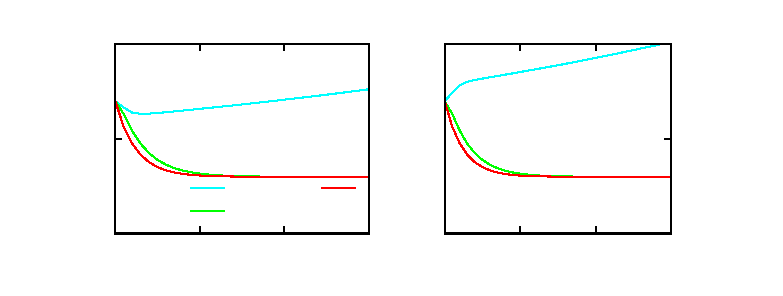
\includegraphics{mpc/unstable_x}}%
    \gplfronttext
  \end{picture}%
\endgroup
}
\resizebox{\textwidth}{!}{% GNUPLOT: LaTeX picture with Postscript
\begingroup
  \makeatletter
  \providecommand\color[2][]{%
    \GenericError{(gnuplot) \space\space\space\@spaces}{%
      Package color not loaded in conjunction with
      terminal option `colourtext'%
    }{See the gnuplot documentation for explanation.%
    }{Either use 'blacktext' in gnuplot or load the package
      color.sty in LaTeX.}%
    \renewcommand\color[2][]{}%
  }%
  \providecommand\includegraphics[2][]{%
    \GenericError{(gnuplot) \space\space\space\@spaces}{%
      Package graphicx or graphics not loaded%
    }{See the gnuplot documentation for explanation.%
    }{The gnuplot epslatex terminal needs graphicx.sty or graphics.sty.}%
    \renewcommand\includegraphics[2][]{}%
  }%
  \providecommand\rotatebox[2]{#2}%
  \@ifundefined{ifGPcolor}{%
    \newif\ifGPcolor
    \GPcolortrue
  }{}%
  \@ifundefined{ifGPblacktext}{%
    \newif\ifGPblacktext
    \GPblacktexttrue
  }{}%
  % define a \g@addto@macro without @ in the name:
  \let\gplgaddtomacro\g@addto@macro
  % define empty templates for all commands taking text:
  \gdef\gplbacktext{}%
  \gdef\gplfronttext{}%
  \makeatother
  \ifGPblacktext
    % no textcolor at all
    \def\colorrgb#1{}%
    \def\colorgray#1{}%
  \else
    % gray or color?
    \ifGPcolor
      \def\colorrgb#1{\color[rgb]{#1}}%
      \def\colorgray#1{\color[gray]{#1}}%
      \expandafter\def\csname LTw\endcsname{\color{white}}%
      \expandafter\def\csname LTb\endcsname{\color{black}}%
      \expandafter\def\csname LTa\endcsname{\color{black}}%
      \expandafter\def\csname LT0\endcsname{\color[rgb]{1,0,0}}%
      \expandafter\def\csname LT1\endcsname{\color[rgb]{0,1,0}}%
      \expandafter\def\csname LT2\endcsname{\color[rgb]{0,0,1}}%
      \expandafter\def\csname LT3\endcsname{\color[rgb]{1,0,1}}%
      \expandafter\def\csname LT4\endcsname{\color[rgb]{0,1,1}}%
      \expandafter\def\csname LT5\endcsname{\color[rgb]{1,1,0}}%
      \expandafter\def\csname LT6\endcsname{\color[rgb]{0,0,0}}%
      \expandafter\def\csname LT7\endcsname{\color[rgb]{1,0.3,0}}%
      \expandafter\def\csname LT8\endcsname{\color[rgb]{0.5,0.5,0.5}}%
    \else
      % gray
      \def\colorrgb#1{\color{black}}%
      \def\colorgray#1{\color[gray]{#1}}%
      \expandafter\def\csname LTw\endcsname{\color{white}}%
      \expandafter\def\csname LTb\endcsname{\color{black}}%
      \expandafter\def\csname LTa\endcsname{\color{black}}%
      \expandafter\def\csname LT0\endcsname{\color{black}}%
      \expandafter\def\csname LT1\endcsname{\color{black}}%
      \expandafter\def\csname LT2\endcsname{\color{black}}%
      \expandafter\def\csname LT3\endcsname{\color{black}}%
      \expandafter\def\csname LT4\endcsname{\color{black}}%
      \expandafter\def\csname LT5\endcsname{\color{black}}%
      \expandafter\def\csname LT6\endcsname{\color{black}}%
      \expandafter\def\csname LT7\endcsname{\color{black}}%
      \expandafter\def\csname LT8\endcsname{\color{black}}%
    \fi
  \fi
  \setlength{\unitlength}{0.0500bp}%
  \begin{picture}(7200.00,2520.00)%
    \gplgaddtomacro\gplbacktext{%
      \csname LTb\endcsname%
      \put(682,803){\makebox(0,0)[r]{\strut{} 0}}%
      \put(682,2256){\makebox(0,0)[r]{\strut{} 2}}%
      \put(814,220){\makebox(0,0){\strut{} 0}}%
      \put(1670,220){\makebox(0,0){\strut{} 10}}%
      \put(2527,220){\makebox(0,0){\strut{} 20}}%
      \put(3383,220){\makebox(0,0){\strut{} 30}}%
      \put(176,1348){\rotatebox{-270}{\makebox(0,0){\strut{}Tank-1 Cheap input}}}%
    }%
    \gplgaddtomacro\gplfronttext{%
    }%
    \gplgaddtomacro\gplbacktext{%
      \csname LTb\endcsname%
      \put(4109,220){\makebox(0,0){\strut{} 0}}%
      \put(4877,220){\makebox(0,0){\strut{} 10}}%
      \put(5646,220){\makebox(0,0){\strut{} 20}}%
      \put(6414,220){\makebox(0,0){\strut{} 30}}%
      \put(6546,803){\makebox(0,0)[l]{\strut{} 0}}%
      \put(6546,1530){\makebox(0,0)[l]{\strut{} 1}}%
      \put(6546,2256){\makebox(0,0)[l]{\strut{} 2}}%
      \put(7051,1348){\rotatebox{-270}{\makebox(0,0){\strut{}Tank-1 Expensive input}}}%
    }%
    \gplgaddtomacro\gplfronttext{%
    }%
    \gplbacktext
    \put(0,0){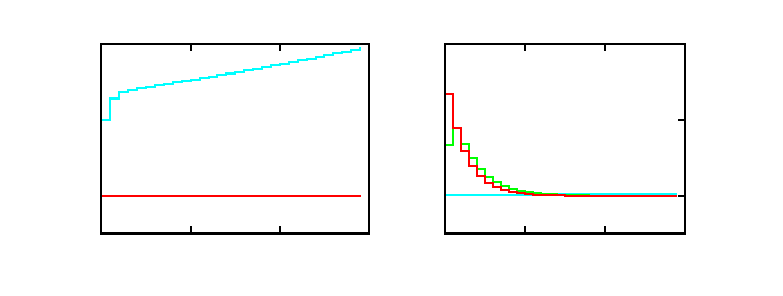
\includegraphics{mpc/unstable_u1}}%
    \gplfronttext
  \end{picture}%
\endgroup
}
\resizebox{\textwidth}{!}{% GNUPLOT: LaTeX picture with Postscript
\begingroup
  \makeatletter
  \providecommand\color[2][]{%
    \GenericError{(gnuplot) \space\space\space\@spaces}{%
      Package color not loaded in conjunction with
      terminal option `colourtext'%
    }{See the gnuplot documentation for explanation.%
    }{Either use 'blacktext' in gnuplot or load the package
      color.sty in LaTeX.}%
    \renewcommand\color[2][]{}%
  }%
  \providecommand\includegraphics[2][]{%
    \GenericError{(gnuplot) \space\space\space\@spaces}{%
      Package graphicx or graphics not loaded%
    }{See the gnuplot documentation for explanation.%
    }{The gnuplot epslatex terminal needs graphicx.sty or graphics.sty.}%
    \renewcommand\includegraphics[2][]{}%
  }%
  \providecommand\rotatebox[2]{#2}%
  \@ifundefined{ifGPcolor}{%
    \newif\ifGPcolor
    \GPcolortrue
  }{}%
  \@ifundefined{ifGPblacktext}{%
    \newif\ifGPblacktext
    \GPblacktexttrue
  }{}%
  % define a \g@addto@macro without @ in the name:
  \let\gplgaddtomacro\g@addto@macro
  % define empty templates for all commands taking text:
  \gdef\gplbacktext{}%
  \gdef\gplfronttext{}%
  \makeatother
  \ifGPblacktext
    % no textcolor at all
    \def\colorrgb#1{}%
    \def\colorgray#1{}%
  \else
    % gray or color?
    \ifGPcolor
      \def\colorrgb#1{\color[rgb]{#1}}%
      \def\colorgray#1{\color[gray]{#1}}%
      \expandafter\def\csname LTw\endcsname{\color{white}}%
      \expandafter\def\csname LTb\endcsname{\color{black}}%
      \expandafter\def\csname LTa\endcsname{\color{black}}%
      \expandafter\def\csname LT0\endcsname{\color[rgb]{1,0,0}}%
      \expandafter\def\csname LT1\endcsname{\color[rgb]{0,1,0}}%
      \expandafter\def\csname LT2\endcsname{\color[rgb]{0,0,1}}%
      \expandafter\def\csname LT3\endcsname{\color[rgb]{1,0,1}}%
      \expandafter\def\csname LT4\endcsname{\color[rgb]{0,1,1}}%
      \expandafter\def\csname LT5\endcsname{\color[rgb]{1,1,0}}%
      \expandafter\def\csname LT6\endcsname{\color[rgb]{0,0,0}}%
      \expandafter\def\csname LT7\endcsname{\color[rgb]{1,0.3,0}}%
      \expandafter\def\csname LT8\endcsname{\color[rgb]{0.5,0.5,0.5}}%
    \else
      % gray
      \def\colorrgb#1{\color{black}}%
      \def\colorgray#1{\color[gray]{#1}}%
      \expandafter\def\csname LTw\endcsname{\color{white}}%
      \expandafter\def\csname LTb\endcsname{\color{black}}%
      \expandafter\def\csname LTa\endcsname{\color{black}}%
      \expandafter\def\csname LT0\endcsname{\color{black}}%
      \expandafter\def\csname LT1\endcsname{\color{black}}%
      \expandafter\def\csname LT2\endcsname{\color{black}}%
      \expandafter\def\csname LT3\endcsname{\color{black}}%
      \expandafter\def\csname LT4\endcsname{\color{black}}%
      \expandafter\def\csname LT5\endcsname{\color{black}}%
      \expandafter\def\csname LT6\endcsname{\color{black}}%
      \expandafter\def\csname LT7\endcsname{\color{black}}%
      \expandafter\def\csname LT8\endcsname{\color{black}}%
    \fi
  \fi
  \setlength{\unitlength}{0.0500bp}%
  \begin{picture}(7200.00,2520.00)%
    \gplgaddtomacro\gplbacktext{%
      \csname LTb\endcsname%
      \put(682,1014){\makebox(0,0)[r]{\strut{} 0}}%
      \put(682,2256){\makebox(0,0)[r]{\strut{} 2}}%
      \put(814,484){\makebox(0,0){\strut{} 0}}%
      \put(1670,484){\makebox(0,0){\strut{} 10}}%
      \put(2527,484){\makebox(0,0){\strut{} 20}}%
      \put(3383,484){\makebox(0,0){\strut{} 30}}%
      \put(176,1480){\rotatebox{-270}{\makebox(0,0){\strut{}Tank-2 Cheap valve}}}%
      \put(2098,154){\makebox(0,0){\strut{}Time}}%
    }%
    \gplgaddtomacro\gplfronttext{%
    }%
    \gplgaddtomacro\gplbacktext{%
      \csname LTb\endcsname%
      \put(4109,484){\makebox(0,0){\strut{} 0}}%
      \put(4877,484){\makebox(0,0){\strut{} 10}}%
      \put(5646,484){\makebox(0,0){\strut{} 20}}%
      \put(6414,484){\makebox(0,0){\strut{} 30}}%
      \put(6546,1014){\makebox(0,0)[l]{\strut{} 0}}%
      \put(6546,1635){\makebox(0,0)[l]{\strut{} 1}}%
      \put(6546,2256){\makebox(0,0)[l]{\strut{} 2}}%
      \put(7051,1480){\rotatebox{-270}{\makebox(0,0){\strut{}Tank-2 Expensive valve}}}%
      \put(5261,154){\makebox(0,0){\strut{}Time}}%
    }%
    \gplgaddtomacro\gplfronttext{%
    }%
    \gplbacktext
    \put(0,0){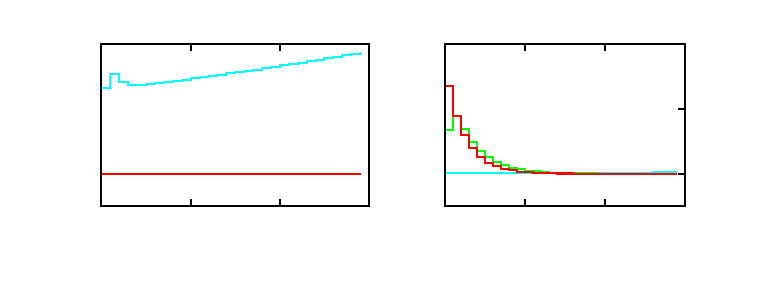
\includegraphics{mpc/unstable_u2}}%
    \gplfronttext
  \end{picture}%
\endgroup
}
\caption{State and input profiles for two-tank system under
  distributed MPC (ncoop: noncooperative, coop: cooperative, cent: centralized).}
\label{fig:unstable}
\end{figure*}
We  wish to keep these control related choices in mind when we develop decompositions of the overall (centralized) problem:
\begin{itemize}
\item All the iterates of the decomposition are feasible and decrease the value function. We need this requirement to be able to use suboptimal MPC theory to establish closed-loop properties.
\item The subsystem MPC problems have similar complexity as the noncoopertive or decentralized MPC problems. 
\item The subsystem MPC problems are independent of each-other. We impose this requirement to ensure that (i) Plant operations continue even if one of the subsystem MPC's stop working  (ii) The subsystem MPC's do not rely on an coordinating layer.
\item If allowed to iterate to convergence, the cooperative MPC input converges to the centralized MPC input. We chose this performance measure because the centralized MPC is the benchmark solution to which all distributed MPC solutions are compared. 
\end{itemize}

\subsection{Cooperative MPC algorithm}
As in the previous section, let  $\mathbb{P}(x)$ represent, any one of the three MPC optimization problems $\mathbb{P}_T(x),\mathbb{P}_N^{\mathbb{F}}(x)$ or $\mathbb{P}_N^{\mathbb{X}_f(a)}(x)$. We remove the state dynamics equality constraints by substitution.  Therefore,  $V(\bu;x)$ represents the corresponding cost function. Without loss of generality, we represent the terminal constraint, i.e., $x(N) = 0$, $x(N) \in \mathbb{F}$ or $x(N) \in \mathbb{X}_f(a)$ as $\mathbf{c}(\bu;x) \leq 0$. 

Given a feasible initial state-input pair $(x,\bu_1^p(x),\bu_2^p(x))$, the subsystem optimization problems are:
\begin{align*} \mathbb{P}_1(x;\bu_2^p)&: \min_{\mathbf{v}_1}{V(\mathbf{v}_1,\bu_2^p;x)} \\&\text{~s.t~}  \mathbf{v}_1 \in \mathbf{U}_1, \mathbf{c}(\mathbf{v}_1,\bu_2^p;x) \leq 0 \end{align*}
Similarly, subsystem-$2$ solves
\begin{align*} \mathbb{P}_1(x;\bu_1^p)&:\ min_{\mathbf{v}_2}{V_(\bu_1^p,\mathbf{v}_2;x)}\\& \text{~s.t~}  \mathbf{v}_2 \in \mathbf{U}_2, \mathbf{c}(\bu_1^p,\mathbf{v}_2;x) \leq 0\end{align*}
Denoting $\mathbf{v}_1^o(\bu_2^p,x)$ and $\mathbf{v}_2^o(\bu_1^p,x)$ as the optimal solutions to the subsystem optimization problems, we define the next iterate as
\[ (\bu_1^{p+1}(x),\bu_2^{p+1}(x)) = \omega(\mathbf{v}_1^o(\bu_2^p,x),\bu_2^p)+(1-\omega)(\bu_1^{p},\mathbf{v}_2^o(\bu_1^p,x))\]
in which $\omega \in [0,1]$.

We can continue the optimizations till they converge, or for any $p\geq 0$. The input at the end of the optimization iteration $p$ is $\bu(x) = (\bu_1^{p}(x),\bu_2^{p}(x))$. If we wish to stop optimizations, we inject the first input in the sequence $\bu$ to the plant and obtain the warm start $\bu_i^0(x^+) = (\bu_i^{p}(0),\bu_i^{p}(1),\ldots,K_ix(N)$, in which $K$ is the feedback gain in the terminal region. This distributed optimization algorithm is a Gauss-Jordan type parallel optimization algorithm \citet[Chapter 3]{bertsekas:tsitsiklis:1989}.

The iterates generated by the cooperative MPC algorithm have the following properties \citep{stewart:venkat:rawlings:wright:pannocchia:2010} :
\begin{enumerate}
\item Each iterate $(\bu_1^{p+1},\bu_2^{p+1})$ is feasible. That is $(\bu_1^{p+1},\bu_2^{p+1}) \in \mathcal{U}(x)$.
\item The cost $V(\bu_1^{p+1},\bu_2^{p+1})$ is non-increasing in $p$ and converges as $p \rightarrow \infty$.
\item In addition, if the terminal constraints are uncoupled, that is $\mathbf{c}(\bu,x) \leq 0$ is of the form $\mathbf{c}_1(x,\bu_1) \leq 0$ and $\mathbf{c}_2(x,\bu_2) \leq 0$, then the iterates converge to the overall (centralized) optimal solution of $\mathbb{P}(x)$.
\end{enumerate}

Notice that these are the properties defined in Definition \ref{thm:propO}. While the warm start ensures that $(\bu_1^0(x^+), \bu_2^0(x^+)) \in G(x,\bu)$, Properties (1) and (2) ensure that $(\bu_1^{p}(x^+),\bu_2^{p}(x^+)) \in G(x,\bu)$. Hence, we can use suboptimal MPC to show the stability of cooperative MPC. See  \citep{stewart:venkat:rawlings:wright:pannocchia:2010} for details.   

Observe that the cooperative MPC algorithm satisfies all the
requirements that we outlined the previous section, most notably, the
absence of any coordinator. However, to satisfy the criteria that the
algorithm converges to the centralized solution, we need to ensure
that there are no coupled terminal constraints. For most systems, we
cannot guarantee that the terminal constraints will be uncoupled,
unless we can find a global control-Lyapunov function. A global
control-Lyapunov function $J(x)$ satisfies the following property:
\[ J(x^+) + \ell(x,u) \leq J(x) \quad u = \kappa (x) \qquad \forall x
\in \mathcal{R}^n 
\]
For example, if the matrix $A$ is stable, then $K=0$ and any $P$ that
solves the Lyapunov equation $A'PA+Q=P$ is a global-Lyapunov function
and we do not need to employ coupled-terminal constraints. 


In the following section, we show two techniques to  remove the coupled constraint $\mathbf{c}(x) \leq 0$ from the optimization problem $\mathbb{P}(x)$. The first technique uses a decoupled, possibly non-minimal centralized model to remove the coupled terminal constraint $x(N) = 0$, while the second method uses a relaxation to remove the ellipsoidal terminal constraint $x(N)'Px(N) \leq a$. 

\subsection{Removing the complicating constraints}
\label{sec:relax}
\paragraph{\textbf{``Decoupled'' centralized model.}}
Consider the following decoupled, possibly non-minimal realization of the centralized (minimal) model:
\begin{multline*} \begin{bmatrix}\tx_{11}\\\tx_{12}\\\tx_{21}\\\tx_{22}\end{bmatrix}^+ = \begin{bmatrix}A_{11}& & &\\&A_{12}& & \\&&A_{21}&\\&&&A_{22}\end{bmatrix}\begin{bmatrix}\tx_{11}\\\tx_{12}\\\tx_{21}\\\tx_{22}\end{bmatrix}+\\\begin{bmatrix}\bar{B}_{11}&\\&\bar{B}_{21}\\\bar{B}_{12}&\\&\bar{B}_{22}\end{bmatrix}\begin{bmatrix}u_1\\u_2\end{bmatrix}\end{multline*}
with
\[\begin{bmatrix}x_1\\x_2\end{bmatrix}= \begin{bmatrix}\bar{C
}_{11}& \bar{C}_{12}&&\\&&\bar{C}_{21}&\bar{C}_{22}\end{bmatrix}\begin{bmatrix}\tx_{11}\\\tx_{12}\\\tx_{21}\\ \tx_{22}\end{bmatrix}\]
Such realizations can be obtained using by transforming the centralized model into the Kalman canonical form \citep[p. 270]{antsaklis:michel:1997}. The terminal condition $x_1(N) = 0, x_2(N) = 0$ is now replaced by $\tx = (\tx_{11},\tx_{12},\tx_{21},\tx_{22}) = 0$. Since substates $\tx_{11}$ and $\tx_{21}$ are not affected by input $u_2$, the condition $(\tx_{11},\tx_{21}) = 0$ takes the form $\mathbf{c}_1(\tx_{11},\tx_{21},\bu_1) = 0$. Similarly, the condition $(\tx_{21},\tx_{22})= 0$ takes the form $\mathbf{c}_2(\tx_{21},\tx_{22},\bu_2) = 0$. Hence, the  optimization problem for terminal control can be written as:
\begin{align*} \mathbb{P}_T(x)&: \min_{\bu_1,\bu_2}{V_T(\bu_1,\bu_2;x)} \\&\text{~s.t~}  \mathbf{u}_1 \in \mathbf{U}_1, \mathbf{u}_2 \in \mathbf{U}_2 \\ &\mathbf{c}_1(\bu_1;x) = 0, \mathbf{c}_2(\bu_2;x) = 0 \end{align*}

However, it must be noted that the substate model (the decoupled centralized model) has to satisfy the following assumption for the decomposition to be useful:
\begin{assumption}
\label{ass:cross_stab}
The systems $(\begin{bmatrix}A_{11}&\\&A_{21}\end{bmatrix},\begin{bmatrix}\bar{B}_{11}\\\bar{B}_{21}\end{bmatrix})$, and  $(\begin{bmatrix}A_{12}&\\&A_{22}\end{bmatrix},\begin{bmatrix}\bar{B}_{12}\\\bar{B}_{22}\end{bmatrix})$ are stabilizable, and the systems s $(\begin{bmatrix}A_{11}&\\&A_{21}\end{bmatrix},\begin{bmatrix}\bar{C}_{11}&\bar{C}_{21}\end{bmatrix})$, and  $(\begin{bmatrix}A_{12}&\\&A_{22}\end{bmatrix},\begin{bmatrix}\bar{C}_{12}&\bar{C}_{22}\end{bmatrix})$ are detectable.
\end{assumption}

{\textbf{Remark.}} Assumption \ref{ass:cross_stab} need not be satisfied for centralized systems that are detectable and stabilizable. For example, for the two tank example, both the stabilizability and detectability assumptions fail for the decoupled centralized model, while the original (minimal) centralized model was stabilizable. Hence, Assumption \ref{ass:cross_stab} restricts the class of systems for which we can guarantee convergence of cooperative MPC to the centralized solution for terminal control.

\paragraph{\textbf{Relaxation.}}
 In the relaxed terminal
 region control problem, we relax the constraint $x(N) \in
 \mathbf{X}_f(a)$ in the terminal region control problem by magnifying
 the cost function. The cost function $V_N^\beta(x,\bu)$ is the sum of the $N$ stage costs and a magnified terminal cost, with $\beta \geq 1$ being the magnification factor.
\[V_N^\beta(x,\bu) = \sum_{k-0}^{N-1} \ell(x(k),u(k)) + \beta
V_f(x(N)) \]
Consider the relaxation to optimization problem $\mathbb{P}_N^{\mathbb{X}_f(a)}(x)$, the optimization problem $\mathbb{P}_N^\beta(x;\bar{V},a)$.
\begin{align*} \mathbb{P}_N^{\beta}(x;\bar{V},a) &: \min_{\bu}{V_N^\beta(x,\bu)}\\& \text{~s.t~} x^+ = Ax+Bu,\\& \bu \in \mathbf{U}^N\end{align*}
Note that $\mathbb{P}_N^\beta$ depends on parameters $\bar{V},a$ and
$\beta$. We have discussed the selection of parameter $a$ in Section
\ref{sec:prelim}. Here, we discuss the selection of parameter
$\beta$. The parameter $\bar{V} \geq a $ is an user choice (usually arbitrarily large).

Note that the problem $\mathbb{P}_N^\beta(x;\bar{V},a)$ does not have
coupling constraints, and therefore the cooperative MPC optimizations
for $\mathbb{P}_N^\beta(x;\bar{V},a)$ converges to the optimal cost
$(V_N^\beta)^o(x)$. However, from the point of view of establishing
closed-loop stability and asymptotic properties, we require that the
terminal region constraint $x(N)'Px(N)\leq a$ be satisfied. In order
to do so, we design the region of attraction and select the parameter
$\beta$ is such a way that the terminal region constraint is
automatically satisfied.

Consider the augmented vector $z = (x,\bu)$. For a $\bar{V} >0$ and
$\beta > 1$, we
define the following set:
\[ \mathbb{Z}_N^\beta(\bar{V}) := \set{(x,\bu) \mid \exists \bu \in
\mathbf{U}^N, V_N^\beta \leq \bar{V}}
\]

Denote $\bar{V}/a = \bar{\beta}$. For the choice of $\beta \geq
\bar{beta}$, it can be shown that $z \in \mathbb{Z}_N^\beta(\bar{V})$ implies
that $V_f(x(N)) \leq a$ as mentioned in the following proposition.

\begin{proposition}
\label{prop:betabar}
Let the cost function be given by $V_N^{\beta}(x,\bu)$. For  $\bar{V}
\geq a $, define $\bar{\beta} := \bar{V}/a)$. Then, for any $\beta \geq \bar{\beta}$ and $(x,\bu) \in \mathbb{Z}_N^\beta(\bar{V})$, we have that $\phi(N;x,\bu) \in \mathbb{X}_f$. 
\end{proposition}
 The proof is by contradiction and  using the fact
that the stage costs and the terminal costs are positive definite.
\citet{pannocchia:rawlings:wright:2011} have also shown that, for a fixed $a>0$, the set
$\mathbb{Z}_N^{\bar{\beta}}(\bar{V})$ approaches the following set
\[ \mathbb{Z}(a) = \set{(x,\bu) \mid \exists \bu \in \mathbf{U}^N,
  \phi(N;x,\bu) \in \mathbb{X}_f}
\]

Therefore, for an initial state $x$, if we chose a initial guess of the
input sequence $\bu \in \mathbf{U}^N$ such that $(x,\bu) \in
\mathbb{Z}_N^{\bar{\beta}}(\bar{V})$, we can ensure that all the input
sequences generated by the cooperative MPC algorithm $\bu^{(p)}$
satisfies  $(x,\bu^{p}) \in \mathbb{Z}_N^{\bar{\beta}}(\bar{V})$,
because the optimization algorithm is non-increasing in the function
value. Hence, every iterate generated by the cooperative MPC algorithm
satisfies the terminal constraint by Proposition \ref{prop:betabar}. 

\textbf{Remark.} Note that the relaxation mentioned in this section is
not an exact relaxation to the problem
$\mathbb{P}_N^{\mathbb{X}_f(a)}$. Therefore, the optimal solution to
$\mathbb{P}^\beta_N(x;\bar{V},a)$ need not be the same as the solution
to $\mathbb{P}_N^{\mathbb{X}_f(a)}$.
 
\textbf{Remark.} It should be noted that the procedure mentioned above to relax the terminal constraint can be used if there is only one terminal constraint. Since a polytopic terminal region like $\mathbb{F}$ consists of more than one inequality constraint, we cannot relax the polytopic terminal region using a terminal cost magnification factor. The ellipsoidal terminal set is a convenient choice for using the relaxation presented in this section. Similarly, the terminal constraint can be viewed as an ellipsoidal terminal region with $a=0$. In such a case, $\beta = \infty$ and the relaxation is not valid. 

\textbf{Remark.} In this section, we discussed two methods to uncouple the terminal constraint. Stability theory for suboptimal MPC, however, require an additional coupled constraint $V(x,\bu) \leq V_f(x), x \in r\mathbb{B}$ or $\bu \leq d\norm{x}, x\in r\mathbb{B}$. As noted earlier, this constraint becomes active only asymptotically as $r>0$ can be chosen arbitrarily small, and therefore is never practically implemented. Therefore, we do not discuss uncoupling this constraint. However, we can show that there exists positive constants $d_1,d_2$ such that $\bu_1 \leq d_1\norm{x}$ and $\bu_2 \leq d_2\norm{x}$, for $x \in r \mathbb{B}$ satisfies $V(x,\bu) \leq V_f(x), x \in r\mathbb{B}$ for linear systems with positive definite $Q,R$ penalty matrices in the stage cost. 

\subsection{Giving up on optimality--Performance measures}
In the previous section, we discussed two modifications to the
optimization problems solved on-line in cooperative MPC that removes
the coupled terminal constraint and thus, ensures that the cooperative
MPC optimizations converge to the centralized solution. However, the
two modifications mentioned converge to the centralized solutions of
two different centralized MPC optimization problems, namely the
terminal constraint problem and a relaxed version of the terminal
region problem. But, if we had the ability to solve a centralized
problem instead, we would have solved the terminal region problem
$\mathbb{P}_N^{\mathbb{F}}$ or $\mathbb{P}_N^{\mathbb{X}_f(a)}$, since
they have the larger region of attraction. If we use
$\mathbb{P}_N^{\mathbb{F}}$ or $\mathbb{P}_N^{\mathbb{X}_f(a)}$
directly in the cooperative MPC optimization, we still retain the
close-loop properties, but we cannot make any guarantees about the
converged solution. The following table shows the average gap between 
(i) The converged $\mathbb{P}_N^\beta(x;\bar{V},a)$ solution and the
solution to $\mathbb{P}_N^{\mathbb{F}}(x)$ and, (ii) the average gap
between the converged cooperative optimization solution to
$\mathbb{P}_N^{\mathbb{F}}(x)$ and the optimal solution to the same
problem. The averages were performed over a grid of the state-space 
that was an approximation of the region of attraction of
$\mathbb{P}_N^\mathbb{F}$.

\begin{table}
\label{tab:optimality_gap}
\caption{Average gap from optimal solution of
  $\mathbb{P}_N^{\mathbb{F}}(x)$}
\centering
\begin{tabular}{l|ccc}
\hline
$\beta$&1&10&20\\
${V}_N^{\beta,o}-{V}_N^{\mathbb{F},o}$&0&10.67&13.98\\
${V}_N^{\mathbb{F},\text{coop}}-V_N^{\mathbb{F},o}$&0&0.025&0.26\\ \hline
\end{tabular}
\end{table}
[Jim: I will convert this into percentages later]

As already mentioned previously, the major issue with using the
``sub-state'' models for cooperative MPC is that the sub-state models
might not satisfy the stabilizability assumptions for centralized
systems that can be stabilized. Therefore, the family of problems for
which the sub-state model is applicable is restricted.

Another issue with the relaxation is that the region of attraction of the controller depends
on $\bar{V}$ and we need to use large values of $\bar{V}$, which
affects the optimization as it makes the Hessian badly
conditioned. The following table shows the number of iterations
required to achieve convergence as a function of the parameter
$\beta$. Note that as the value of $\beta$ increases, the condition
number of the Hessian increases, indicating that the step-size taken
by the cooperative MPC algorithm will become smaller and smaller as
$\beta$ increases. 
\begin{table}
\centering
\caption{Impact of $\beta$: 2 tanks problem}
\label{tab:beta_tank}
\begin{tabular}{l|cccc}\hline
&$\beta=1$&$\beta=10$&$\beta=20$ & $\beta=100$\\\hline
Number of iterations&535&2548&4825&23069\\
Condition number&70&338&640&3065\\
\end{tabular}
\end{table}


We also compare the closed-loop performance when doing only one
iteration of the cooperative MPC algorithm. When we just do one
iteration of the algorithm, we cannot make any guarantees about the
quality of the first descent direction generated by the algorithms.
\begin{table*}
\centering
\caption{Closed loop performance-2 tank problem}
\label{tab:loss_tank_cl}
\begin{tabular}{l|cccc}\hline
& 1 iteration & Convergence & 1 iteration & Convergence\\
Problem & $x(N) \in \mathbb{F}$&$x(N) \in \mathbb{F}$& $V_N^{200}$ &
$V_N^{200}$\\\hline
$x= x_1$& 2.42&0.33&2.66&0.28\\
$x= x_2$& 3.5&1.19&16&22\\
$x= x_3$& 7.2&0.11&21.54&16.4\\
$x= x_4$& 2.3&0.11&3.09&0.25\\
\hline
\end{tabular}
\end{table*}

[Jim: I will rerun the simulations for beta=20]

Finally, we also comment on the issue of initialization/
re-initialization. All the methods that we mentioned for cooperative
MPC requires that we start from an feasible initial $(x,\bu)$
pair. However, it may so happen that disturbances may make the warm
start infeasible for the successor state.  To ensure robustness to
disturbances, we must have a method to cooperatively  re-initialize the system
whenever the warm start fails. The problem therefore, is to find a
feasible point in the intersection of convex sets. Parallel algorithms
for projecting onto convex sets generally find a feasible point upon
convergence \citep{bauschke:borwein:1996}. Hence, for the case in which we solve
$\mathbb{P}_N^{\mathbb{F}}$ or $\mathbb{P}_N^{\mathbb{X}_f(a)}$
directly, the restart algorithm has to be centralized. On the other
hand, if for the sub-state models, as the terminal constraints are
uncoupled, each sub-system can independently find a restart point if
the warm start fails. If we use the relaxation formulation, then
notice that by design of the optimization problem, whenever the cost
$V_N^\beta(x,\bu)$ falls below $\bar{V}$, the terminal condition is
satisfied. Therefore, when the warm-start fails, the two subsystems
can continue to still perform the same optimizations that they would
do in the nominal case; the only difference being that they have to
iterate till the cost drops below $\bar{V}$. In general, we cannot
provide any guarantees on the number of iterations required to recover
feasibility, but for small disturbances, we recover feasibility within
a few iterations. To generate the following table, we randomly
selected  $1000$  initial input sequences that were infeasible, that
is $(x,\bu) \notin \mathbb{Z}_N^{\beta}(\bar{V})$. For each such
infeasible sequence, we counted the number of cooperative iterations
that was needed to recover feasibility. This experiment was repeated
for a number of initial states in the admissible region. The maximum
and the average number of iterations required to recover feasibility
is reported in the following table along with the worst and average
cost function value.
\begin{table}
\label{tab:recovery}
\begin{center}
\begin{tabular}{p{0.2\textwidth}|ccc}
 \hline
 $\beta$& 1 & 20& 100 \\
 Average no. of iterations & 2.4&1.5&1.5\\
 Maximum no. of iterations & 10 & 5 & 17\\
 Average $V-\bar{V}$ & 609&7445&34445 \\
 Maximum $V-\bar{V}$& 1257&22249&96319 \\
 \hline
\end{tabular}
\end{center}
\end{table}


The following table is a summary of the observations made in this  section.
\begin{table*}
 \label{tab:summary}
 \begin{center}
  %\renewcommand{\arraystretch}{1.4}
  
  
  \begin{tabular}{|p{0.2\textwidth}|p{0.2\textwidth}p{0.2\textwidth}p{0.2\textwidth}|}\hline\hline
   &Sub-state&Relaxation&Centralized\\ \hline
   Terminal Region & $x(N) = 0$ & $V_f(x(N))\leq a$& 
$\mathbb{X}_f(a)
   or \mathbb{F}$\\ \hline
   Stability & \multicolumn{3}{c}{By design using {suboptimal MPC}}\\ \hline
   Convergence & Converges to centralized $x(N)=0$& Converges to centralized relaxed&Gets stuck on boundary \\ \hline
   Convergence to \textit{Centralized}&No&No&No  \\ \hline
   Restart&Distributed; {Independent}& Distributed; {subsystems need
     to iterate}&Centralized; or parallel iterated to convergence \\ \hline
   Applicability& {Restricted}&\multicolumn{2}{c}{{To all stabilizable systems}} \\ \hline
   Region of Attraction& $\mathcal{X}_N^T$\hfill $ \subseteq$&$\mathcal{X}_{N}^{{\beta}}$\hfill$\subseteq$&$\mathcal{X}_N$\\
   \hline
   \hline
   \end{tabular}
 \end{center} 
\end{table*}


\section{Conclusions and Future work}
\begin{itemize}
\item Cooperative versus Parallel : Comment about finding
  decompositions to ``tough' centralized nonlinear problems, that
  could have the structure of multiple MPC's, but having that
  structure is not necessary (better decompositions may exist if we
  partition the inputs differently etc).
  \textbf{somehow debate that cooperative is more about maintaining
    the individuality of the controllers}
\item Can we stabilize Noncooperative games? Particular interest to
  supply chains
\end{itemize}
\bibliographystyle{abbrvnat}
{\scriptsize
\bibliography{abbreviations,articles,proceedings,books,unpub}
}
\end{document}
\newpage
\section*{Mathematical notation (to be removed before submission)}

\subsection*{Section-2}
\begin{notation}{$\Inv_i(k)$}
\sym{\I} The set of node
\sym{\mathcal{R}} Set of Retailers.
\sym{\mathcal{M}} Set of manufacturers
\sym{\UP(i)}  Set of nodes $j \in \I$ which are upstream to
node $i \in \I$.
\sym{\DN(i)}  Set of nodes $j \in \I$ which are downstram to
node $i \in \I$.
\sym{\Inv_i(k)} Inventory in node $i$, $i \in \I$ at discrete time $k$
\sym{\BO_i(k)} Back Order in node $i$, $i \in \I$ at discrete time $k$
\sym{S_{ij}} Amount shipped by node $i$ to node $j$, $i,j \in \I$.
\sym{O_{ij}} Orders placed by node $i$ to node $j$, $i,j \in \I$.
\sym{\tau_{ij}} The shipment delay between node $i$ and node $j$. $i,j
\in \I$.
\sym{S_{ic}} Shipment made by node $i \in \mathcal{R}$ to customer.
\sym{\Dem_{ic}} Demand at retailer node $i \in \mathcal{R}$.
\sym{S_{ip}} Amount produces by node $i \in \mathcal{M}$.
\sym{\tau_{ip}} Production delay at node $i \in \mathcal{M}$.
\sym{\IP_i}   Inventory position at node $i \in \I$.
\sym{x}       States: Inventories and back orders in each node
\sym{u}       Inputs: Shipments and orders in each node
\sym{d}       Disturbances: Customer demands
\sym{(A,B,B_d)}   Dynamic system matrices
\end{notation}

\subsection*{Section-3,4,5}
\begin{notation}{$V_N^{\beta}(x,\bu_1,\bu_2)$}
\sym{\mathbb{I}_{a:b}} Set of integers from $a$ to $b$, $a<b$.
\sym{\mathbb{X}} State constraint set
\sym{\mathbb{X}_f} Terminal set
\sym{\mathbb{U}_i} The constraint set for input $i$.
\sym{\mathbb{U}}  Input constraint set
\sym{\mathbb{Z}_N} Set of feasible inital state-input sequence pairs.
\sym{\mathcal{U}_N(x)} Set of feasible input sequence for state $x$
and problem $\mathbb{P}(x)$.
\sym{\mathbb{Z}^\beta_N} Set of feasible inital state-input sequence pairs.
\sym{\mathcal{U}^\beta_N(x)} Set of feasible input sequence for state $x$
and problem $\mathbb{P}^\beta(x)$.

\sym{\mathcal{B}_r} Ball of radius $r>0$.

\sym{x} The state of the system (centralized)
\sym{u_i} The inputs which can be manipulated by subsystem- $i$.
\sym{\bu} $=(u(0),u(1),\ldots,u(N-1))$; vector of inputs
\sym{\tilde{\bu}} Warm start
\sym{\phi(i;x,\bu)} The state at time $i\geq 0$ starting from $x$ at
time $0$ under input $\bu$
\sym{N}  The control/prediction horizon.
\sym{\eig(Q)} Set of eigenvalues of matrix $Q$.
\sym{\olambda(Q)} Largest eigenvalue of positive definite matrix $Q$.
\sym{\ulambda(Q)} Smallest eigenvalue of positive definite matrix $Q$.
\sym{p} Optimization iterate, noncooperative and cooperative MPC
\sym{A}  The (centralized) state evolution matrix
\sym{B_{i}} The matrix describing the influence of input $i$ on the
states.
\sym{Q} State penalty matrix
\sym{Q_i} State penalty matrix for subsystem-$i$, Noncooperative MPC
\sym{R_i} Input penalty matrix for input $i$
\sym{P} Terminal penalty matrix
\sym{P_i} Terminal penalty matrix for subsystem-$i$, Noncooperative
MPC
\sym{\mathcal{\kappa}(\cdot)} Stabilizing controller $u = \kappa(x)$ in terminal region $\mathbb{X}_f$.
\sym{K} Linear stablilizing controller $u = Kx$ in terminal region $\mathbb{X}_f$.
\sym{\ell^i(x,u_i)} Stage cost for subsystem-$i$
\sym{V_f^{i}(x)} Terminal cost for subsystem-$i$, Noncooperative MPC
\sym{V_f(x)} Terminal cost
\sym{V_N^i(x,\bu_i)} Cost function for subsystem-$i$, Noncooperative MPC
\sym{V_N(x,\bu_1,\bu_2)} Cost function, Cooperative and Centralized
MPC\sym{V_N^{i,\beta}(x,\bu_i)} Cost function for subsystem $i$ with
terminal penalty $\beta V_f^{i,\beta}$, Noncooperative MPC
\sym{V_N^{\beta}(x,\bu_1,\bu_2)} Cost function with terminal penalty
$\beta V_f(x)$, Cooperative and Centralized
MPC

\sym{\mathbb{P}(x)} Centralized MPC problem with cost function
$V_N(x,\bu)$
\sym{\mathbb{P}^\beta(x)} Centralized MPC problem with cost function
$V^\beta_N(x,\bu)$
\sym{\mathbb{P}_i^{nc}(x_i,\bu_j^s)} Noncooperative MPC problem for subsystem $i$
with cost function $V_N^{i,\beta}$ and $\bu_j^s, j \neq i$ being the
shared input.
\sym{\mathbb{P}_i^{c}(x,\bu_j^{s})} Cooperatve MPC problem for subsystem $i$ with
cost function $V_N^\beta$ and $\bu_j^s, j \neq i$ being the
shared input.
\end{notation}

\end{document}
